\begin{Large} 
	\textbf{Задача 1}\\
	
	 \end{Large} 
Задача заключалась в реализации следующих функий в классе: (был выбран ЯП Python, полный листинг кода см. в приложении А)
\begin{itemize}
	\item Ввод матрицы заданного размера пользователем.
	\item Подсчет следа матрицы.
	\item Поиск и вывод элемента матрицы по заданным индексам.
	\item Тестирование работы программы и создание консольного пользовательского интерфейса.\\
\end{itemize}

\begin{large}
	Использованные библиотеки и инструменты языка\\
\end{large}
В ходе написания программы были использованы только стандартные средства языка. Также для удобства и лучшей читаемости кода была импортирована библиотека typing.\\

\begin{large}
	Реализация функций и основные идеи\\
\end{large}
Все функции были реализованы в классе MatrixKeeper\\\\
Написаны функции:\\
1. inputMatrix - ввод матрицы пользователем,\\
2. trace - поиск следа матрицы,\\
3. findByIndex - поиск элемента по введенному индексу.\\

Суть работы алгоритмов:
\begin{itemize}
	\item inputMatrix: Приглашение пользователя ко вводу. Вначале через пробел вводятся два числа типа int - размер матрицы. Вторым приглашением вводится матрица по строке, элементы в строке разделяются пробелом.
	\item trace: След матрицы - сумма элементов главной диагонали этой матрицы. Циклом, оставаясь в пределах матрицы, проходимся по элементам с индексами вида [i][i], считаем сумму таких элементов. Можем так делать по той причине, что матрица имеет следующую структуру в классе:\vspace{3cm}
	\begin{lstlisting} [language=Python]
		self.matrix: Optional[List[List[float]]]
		\end{lstlisting} - то есть храним матрицу как список, каждый элемент которого является тоже списком.
	\item findByIndex: возвращаем элемент из матрицы, отнимая от индексов по единице, т.к. в ЯП отсчет начинается с нуля.
	\begin{lstlisting}
		return self.matrix[n-1][m-1]
	\end{lstlisting}
\end{itemize}
\begin{large}
	Тестирование программы\\
\end{large}
Написаны юниттесты для каждой функции класса с помощью стандартной библиотеки unittest. Также протестировано вручную.\\
Листинг кода теста см. в приложении А-test.\\
\begin{figure}[H]
	\centering
	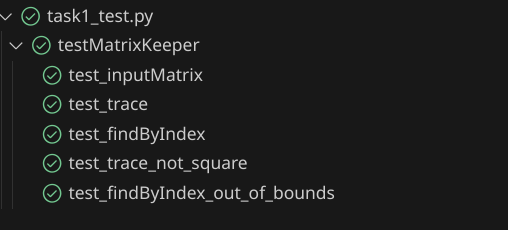
\includegraphics[width=0.5\linewidth]{tests-task1}
	\caption*{Успешное прохождение unittests}
	\label{fig:tests-task1}
\end{figure}
\begin{figure}[H]
	\centering
	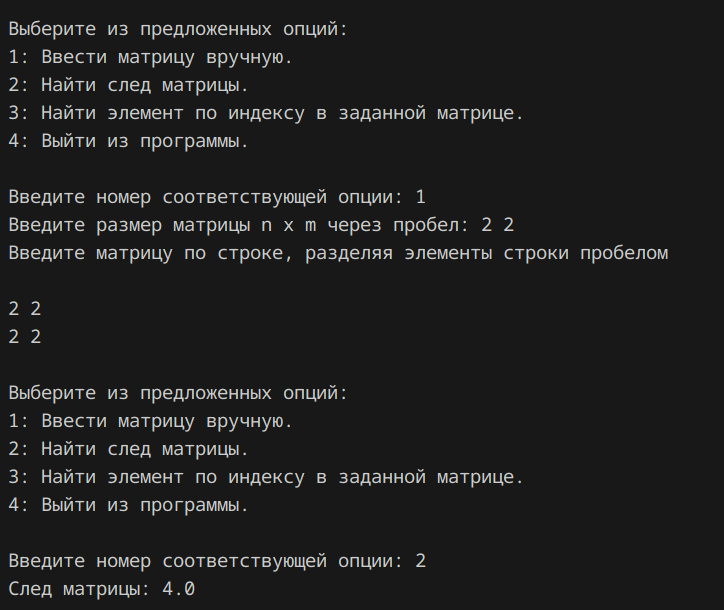
\includegraphics[width=0.5\linewidth]{tests-task2}
	\caption*{Ручной тест поиска следа матрицы 2х2 со всеми элементами, равными 2.}
	\label{fig:tests-task2}
\end{figure}
\begin{figure}[H]
	\centering
	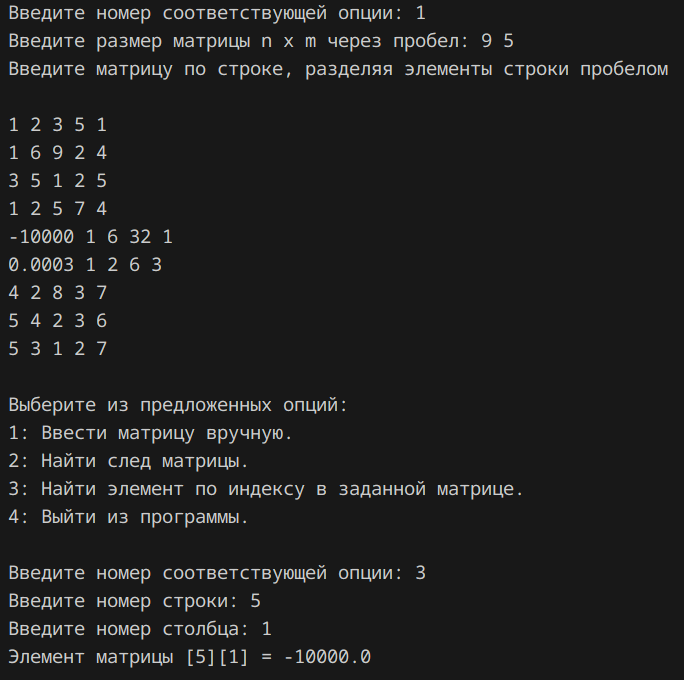
\includegraphics[width=0.5\linewidth]{tests-task3}
	\caption*{Ручной тест поиска страшного элемента в страшной матрице 9х5.}
	\label{fig:tests-task3}
\end{figure}
Итак, справились с первым заданием.\vspace{2cm}

\begin{large}
	Задача 2\\
\end{large}
Во второй задаче требуется реализовать три функции для операций с матрицами: (полный листинг кода см. в приложении Б)\\
\begin{itemize}
	\item Сложение двух матриц.
	\item Умножение двух матриц.
	\item Умножение матрицы на скаляр.\\
\end{itemize}

\begin{large}
	Использованные библиотеки и инструменты языка\\
\end{large}
В ходе написания программы были использованы только стандартные средства языка. Также для удобства и лучшей читаемости кода была импортирована библиотека typing.\\\\
Были реализованы 3 функции:\\
1. matrixAddition - сложение двух матриц.\\
2. matrixByMatrixMultiplication - перемножение двух матриц.\\
3. matrixScalarMultiplication - умножение одной из двух матриц на заданное число.\\
Согласно техническому заданию, функция ввода матрицы пользователем была импортирована из файла предыдущего задания. (inputMatrix)

Суть работы алгоритмов:
\begin{itemize}
	\item \textbf{matrixAddition}: Классическое сложение матрицы. Возвращаем матрицу, где каждый элемент с определенными индексами равен сумме элементов с соответствующими индексами из складываемых матриц.
	\begin{gather*}
		(A+B)_{i,k} = A_{i,k} + B_{i,k}
	\end{gather*}
	
	\item \textbf{matrixByMatrixMultiplication}: Умножение матрицы на матрицу. Возвращаем матрицу, где каждый элемент с определенными индексами равен сумме произведений элементов соответствующей строки первой матрицы и столбца второй матрицы.
	\begin{gather*}
		(AB)_{i,j} = \sum_{k=1}^{n} A_{i,k} \cdot B_{k,j}
	\end{gather*}
	
	\item \textbf{matrixScalarMultiplication}: Умножение матрицы на скаляр. Возвращаем матрицу, где каждый элемент равен произведению соответствующего элемента исходной матрицы и скаляра.
	\begin{gather*}
		(cA)_{i,j} = c \cdot A_{i,j}
	\end{gather*}
\end{itemize}
\begin{large}
	Тестирование программы\\
\end{large}
Написаны юниттесты для каждой функции класса с помощью стандартной библиотеки unittest. Также протестировано вручную.\\
Листинг кода теста см. в приложении Б-test.\\
\begin{figure}[H]
	\centering
	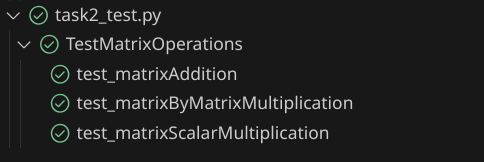
\includegraphics[width=0.5\linewidth]{tests-task4}
	\caption*{Успешное прохождение unittests}
	\label{fig:tests-task4}
\end{figure}
\begin{figure}[H]
	\centering
	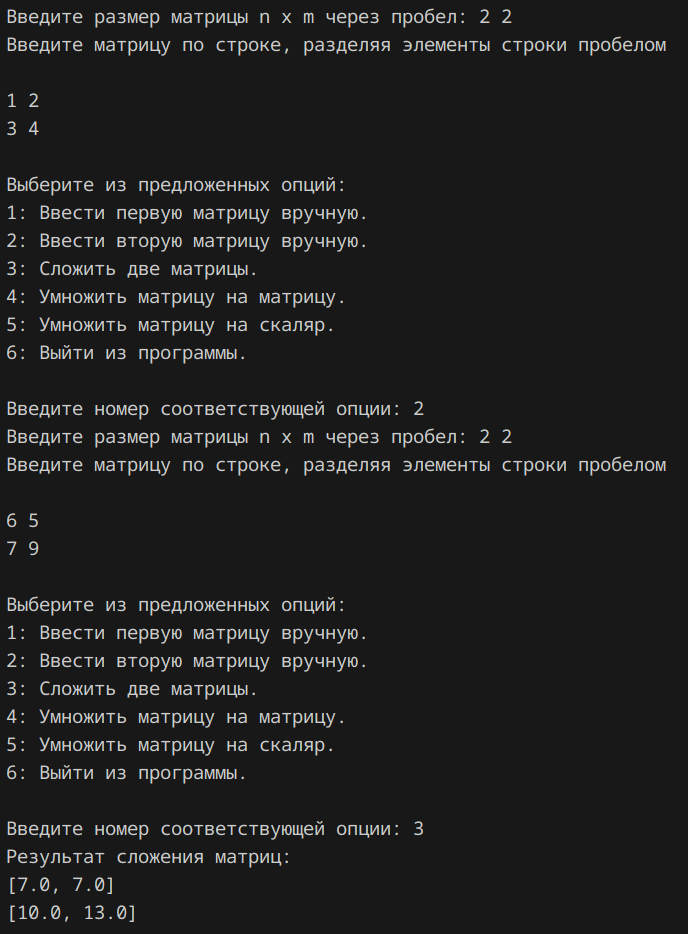
\includegraphics[width=0.46\linewidth]{tests-task5}
	\caption*{Ручной тест сложения двух матриц 2 на 2.}
	\label{fig:tests-task5}
\end{figure}
\begin{figure}[H]
	\centering
	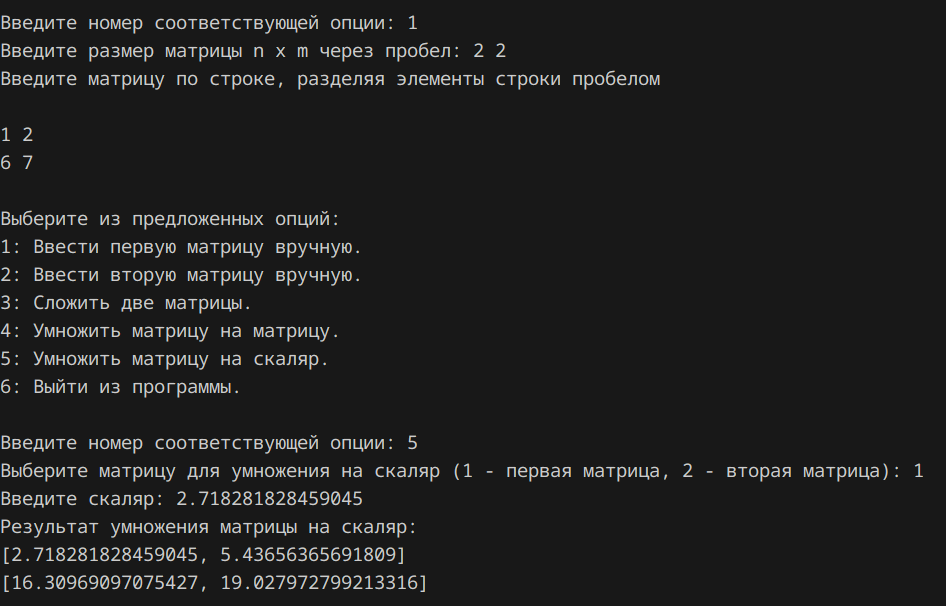
\includegraphics[width=0.58\linewidth]{tests-task6}
	\caption*{Ручной тест умножения матрицы 2 на 2 на число Эйлера с небольшим количеством знаков после запятой.}
	\label{fig:tests-task6}
\end{figure}
\begin{figure}[H]
	\centering
	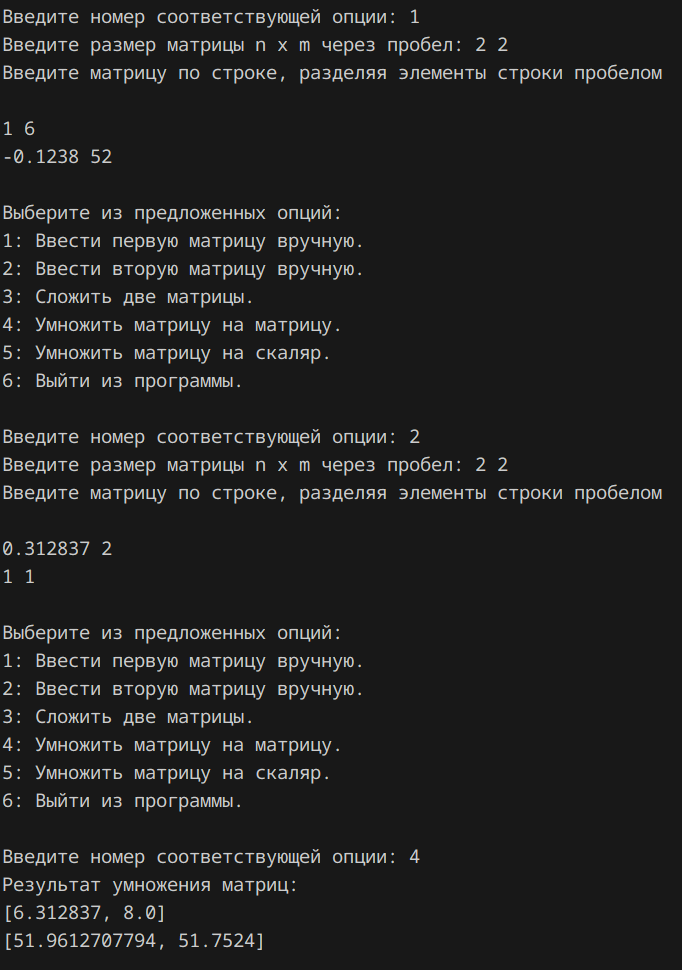
\includegraphics[width=0.7\linewidth]{tests-task7}
	\caption*{Ручной тест умножения двух страшных матриц 2 на 2.}
	\label{fig:tests-task7}
\end{figure}
\begin{figure}[H]
	\centering
	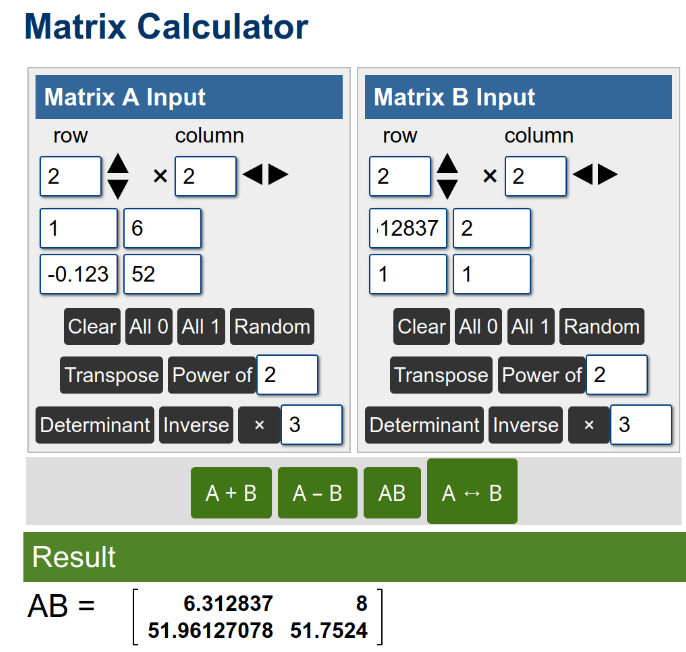
\includegraphics[width=0.5\linewidth]{tests-task8}
	\caption*{Удостоверимся в правильности полученного результата, умножив матрицы на сайте-калькуляторе. Результат правильный.}
	\label{fig:tests-task8}
\end{figure}
Справились со вторым заданием. \vspace{2cm}

\begin{large}
	Задача 3\\
\end{large}
В третьей задача требуется реализовать следующие функции: (полный листинг кода см. в приложении В)
\begin{itemize}
	\item Вычисление определителя матрицы. По тз - матрицы размером до 100х100
	\item Ответ на вопрос: существует ли матрица, обратная данной.
\end{itemize}
\begin{large}
	Использованные библиотеки и инструменты языка\\
\end{large}
В ходе написания программы были использованы только стандартные средства языка. Также для удобства и лучшей читаемости кода была импортирована библиотека typing.\\ \\
Были реализованы 3 функции:\\
1. determinantOfMatrix - поиск определителя матрицы.\\
2. isMatrixInvertable - функция, которая отвечает на вопрос, существует ли обратная матрица к данной.\\
3. gauss - вспомогательная функция - метод Гаусса, с помощью которого считал определитель любой квадратной матрицы.\vspace{2cm}

Суть работы алгоритмов:
\begin{itemize}
	\item determinantOfMatrix: оболочка функции, проверяем размер матрицы и обращаемся к функции Гаусса для поиска определителя.
	\item isMatrixInvertable: сравниваем полученный из первой функции определитель с нулем, возвращаем логическое значение "да" или "нет".
	\item gauss: самая интересная функция. Для матрицы 1х1 и 2х2 посчитано вручную.
	\begin{lstlisting}
		n = len(matrix)
		if n == 1:
			return matrix[0][0] 
		elif n == 2:
			return matrix[0][0] * matrix[1][1] - matrix[0][1] * matrix[1][0] 
	\end{lstlisting}
	1х1: Определитель равен единственному элементу.\\
	2х2: Определитель считаем как разность произведения элементов главной и побочной диагоналей.\\ \\
	Проверка на вырожденную матрицу:
	\begin{lstlisting}
		for i in range(n):
			max_row = max(range(i, n), key=lambda r: abs(matrix[r][i]))
			if matrix[max_row][i] == 0:
				raise ValueError("Matrix is singular, 			determinant is zero.")
	\end{lstlisting}
	
	Как работает:
	
	Цикл проходит по каждому столбцу \texttt{i} от $0$ до $n-1$. На каждом шаге ищется ведущий элемент в текущем столбце. Для этого используется команда:
	
	\begin{lstlisting}
		max_row = max(range(i, n), key=lambda r: abs(matrix[r][i]))
	\end{lstlisting}
	
	Здесь \texttt{range(i, n)} генерирует индексы строк от текущей строки \texttt{i} до последней \texttt{n-1}, \texttt{lambda r: abs(matrix[r][i])} вычисляет модуль элемента в текущем столбце для каждой строки \texttt{r}, а \texttt{max(..., key=...)} выбирает индекс строки \texttt{max\_row}, где модуль элемента в столбце максимален.
	
	Далее выполняется проверка:
	\begin{lstlisting}
		if matrix[max_row][i] == 0:
			raise ValueError("Matrix is singular, determinant is zero.")
	\end{lstlisting}
	
	Если максимальный элемент в столбце равен $0$, то все элементы ниже $i$-й строки в этом столбце тоже равны $0$. Это означает, что матрица вырожденная, и её определитель равен нулю, поэтому дальнейшие вычисления прекращаются.\\ \\
	Приведение к нижнетреугольному виду и вычисление определителя:
	
	Для приведения матрицы к нижнетреугольному виду используется следующий алгоритм. Если строка с максимальным элементом в текущем столбце \texttt{max\_row} не совпадает с текущей строкой \texttt{i}, строки меняются местами:
	
	\begin{lstlisting}
		if max_row != i:
			matrix[i], matrix[max_row] = matrix[max_row], matrix[i]
			swap_count += 1
	\end{lstlisting}
	
	После этого элементы ниже ведущего в текущем столбце обнуляются. Для каждой строки \texttt{j}, начиная с \texttt{i + 1}, вычисляется коэффициент \texttt{factor}, с помощью которого корректируются элементы строки:
	
	\begin{lstlisting}
		for j in range(i + 1, n):
			factor = matrix[j][i] / matrix[i][i]
			for k in range(i, n):
				matrix[j][k] -= factor * matrix[i][k]
	\end{lstlisting}
	
	После завершения приведения к нижнетреугольному виду вычисляется определитель матрицы. Определитель является произведением всех диагональных элементов приведённой матрицы:
	
	\begin{lstlisting}
		determinant = 1.0
		for i in range(n):
			determinant *= matrix[i][i]
	\end{lstlisting}
	
	Учитывается знак определителя, зависящий от числа перестановок строк:
	
	\begin{lstlisting}
		return (-1) ** swap_count * determinant
	\end{lstlisting}
	
	Здесь каждая перестановка строк меняет знак определителя, что учитывается выражением \texttt{(-1) ** swap\_count}.
\end{itemize}
Таким образом реализован метод Гаусса для поиска определителя любой квадратной матрицы.\\ \\
\begin{large}
	Тестирование программы\\
\end{large}
Написаны юниттесты для каждой функции класса с помощью стандартной библиотеки unittest. Также протестировано вручную.\\
Листинг кода теста см. в приложении В-test.\\
\begin{figure}[H]
	\centering
	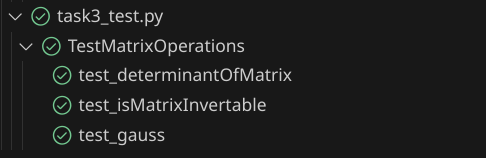
\includegraphics[width=0.5\linewidth]{tests-task9}
	\caption*{Успешное прохождение unittests}
	\label{fig:tests-task9}
\end{figure}
\begin{figure}[H]
	\centering
	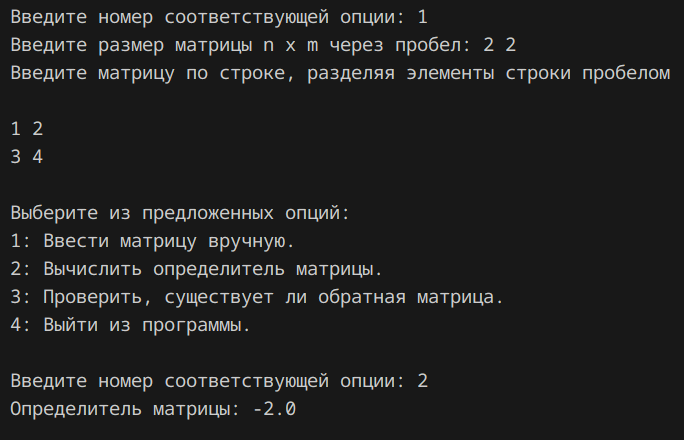
\includegraphics[width=0.5\linewidth]{tests-task10}
	\caption*{Вручную проверям подсчет определителя матрицы 2х2. Ответ верный.}
	\label{fig:tests-task10}
\end{figure}
\begin{figure}[H]
	\centering
	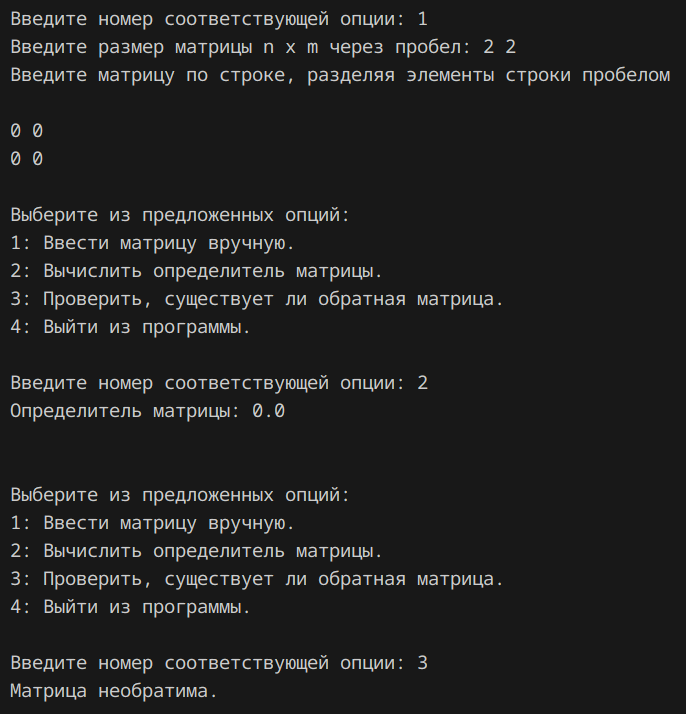
\includegraphics[width=0.5\linewidth]{tests-task11}
	\caption*{Вручную проверяем подсчет определителя и обратимости нулевой матрицы. Ответ верный.}
	\label{fig:tests-task11}
\end{figure}
\begin{figure}[H]
	\centering
	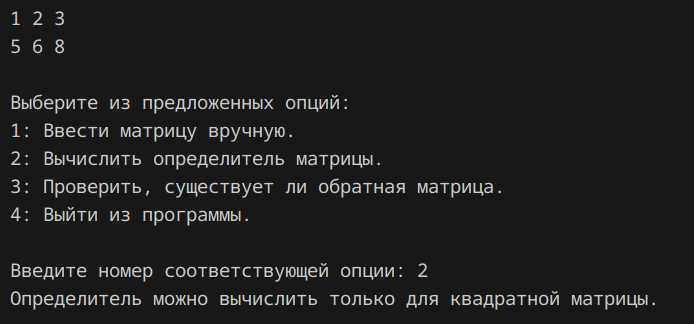
\includegraphics[width=0.5\linewidth]{tests-task12}
	\caption*{Конечно же, вручную пытаемся обработать не квадратную матрицу.}
	\label{fig:tests-task12}
\end{figure}
Итак, все задания сделаны, тесты пройдены. Пора перейти к выводам.


